\section{Simulations for Stationary Strategies}\label{sec:simulations-for-stationary-strategies}
\begin{figure}[h]
    \centering
    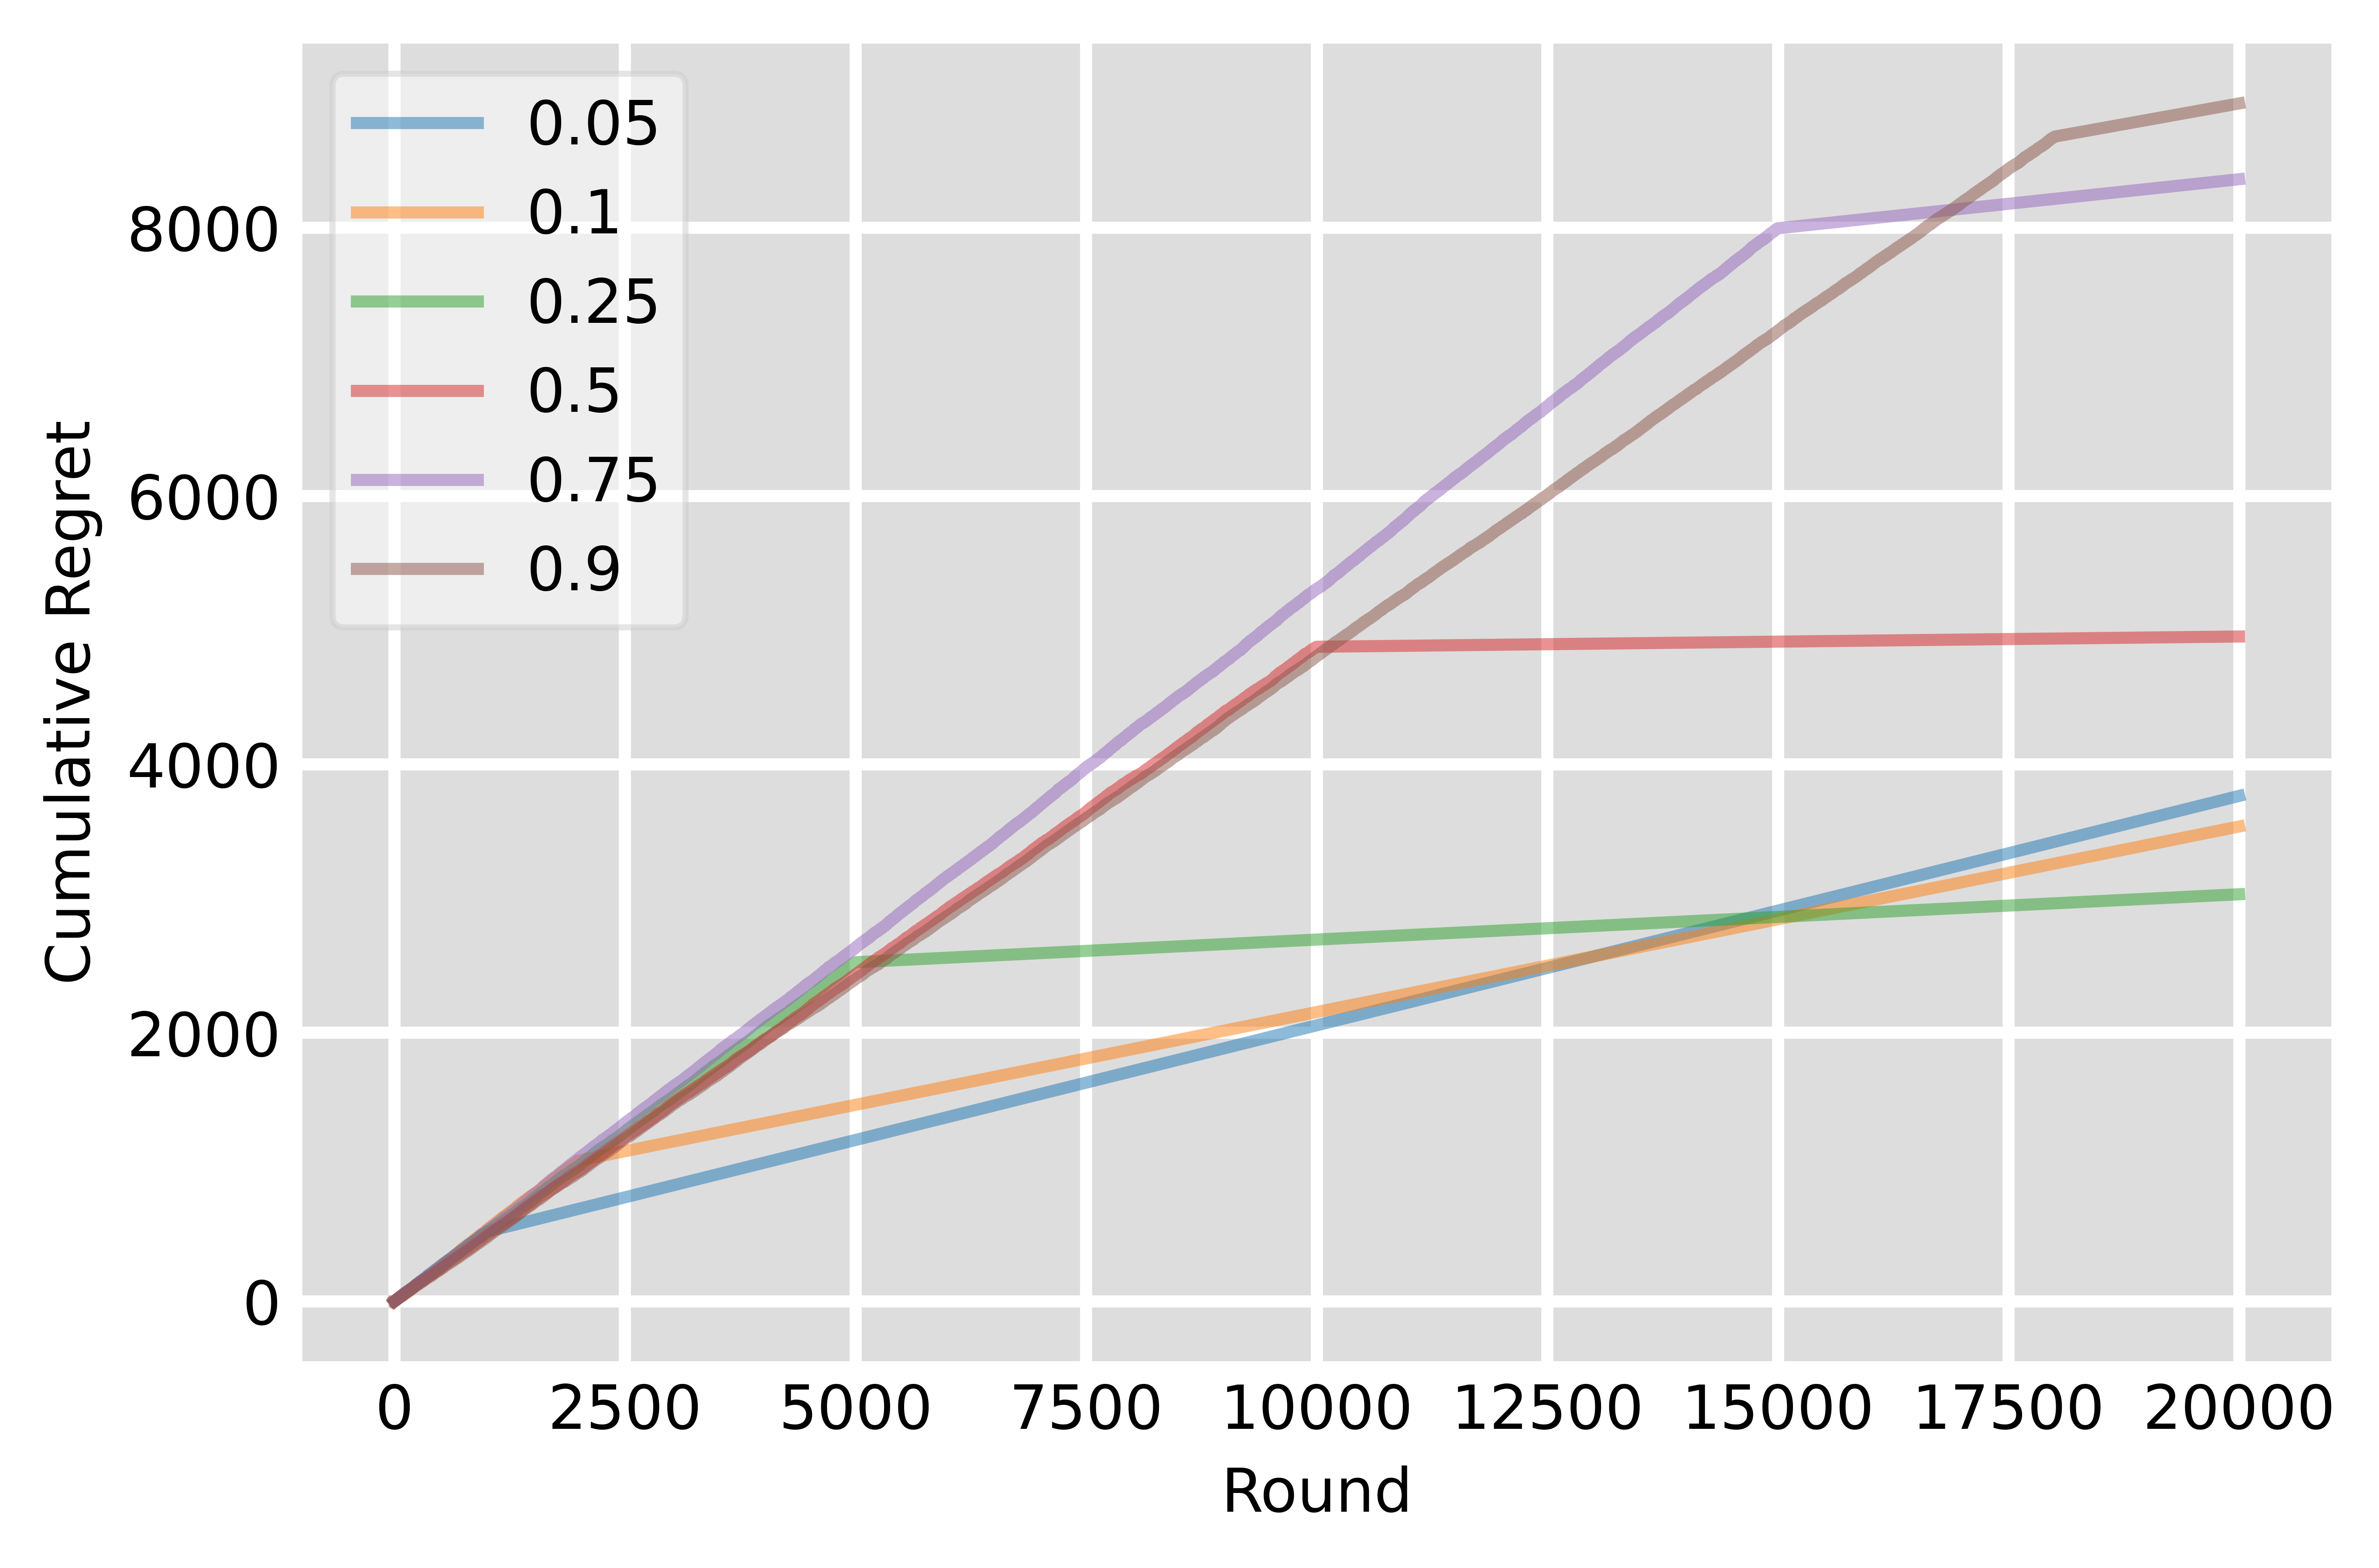
\includegraphics[width=0.9\textwidth]{figures/epsilon_plot.png}
    \caption[Epsilon-first strategy with varying values of epsilon]{Epsilon-first strategy with varying values of epsilon. 100 arms. 20000 rounds per iteration. Average of 50 iterations}
    \label{fig: epsilon}
\end{figure}

\begin{figure}[h]
    \centering
    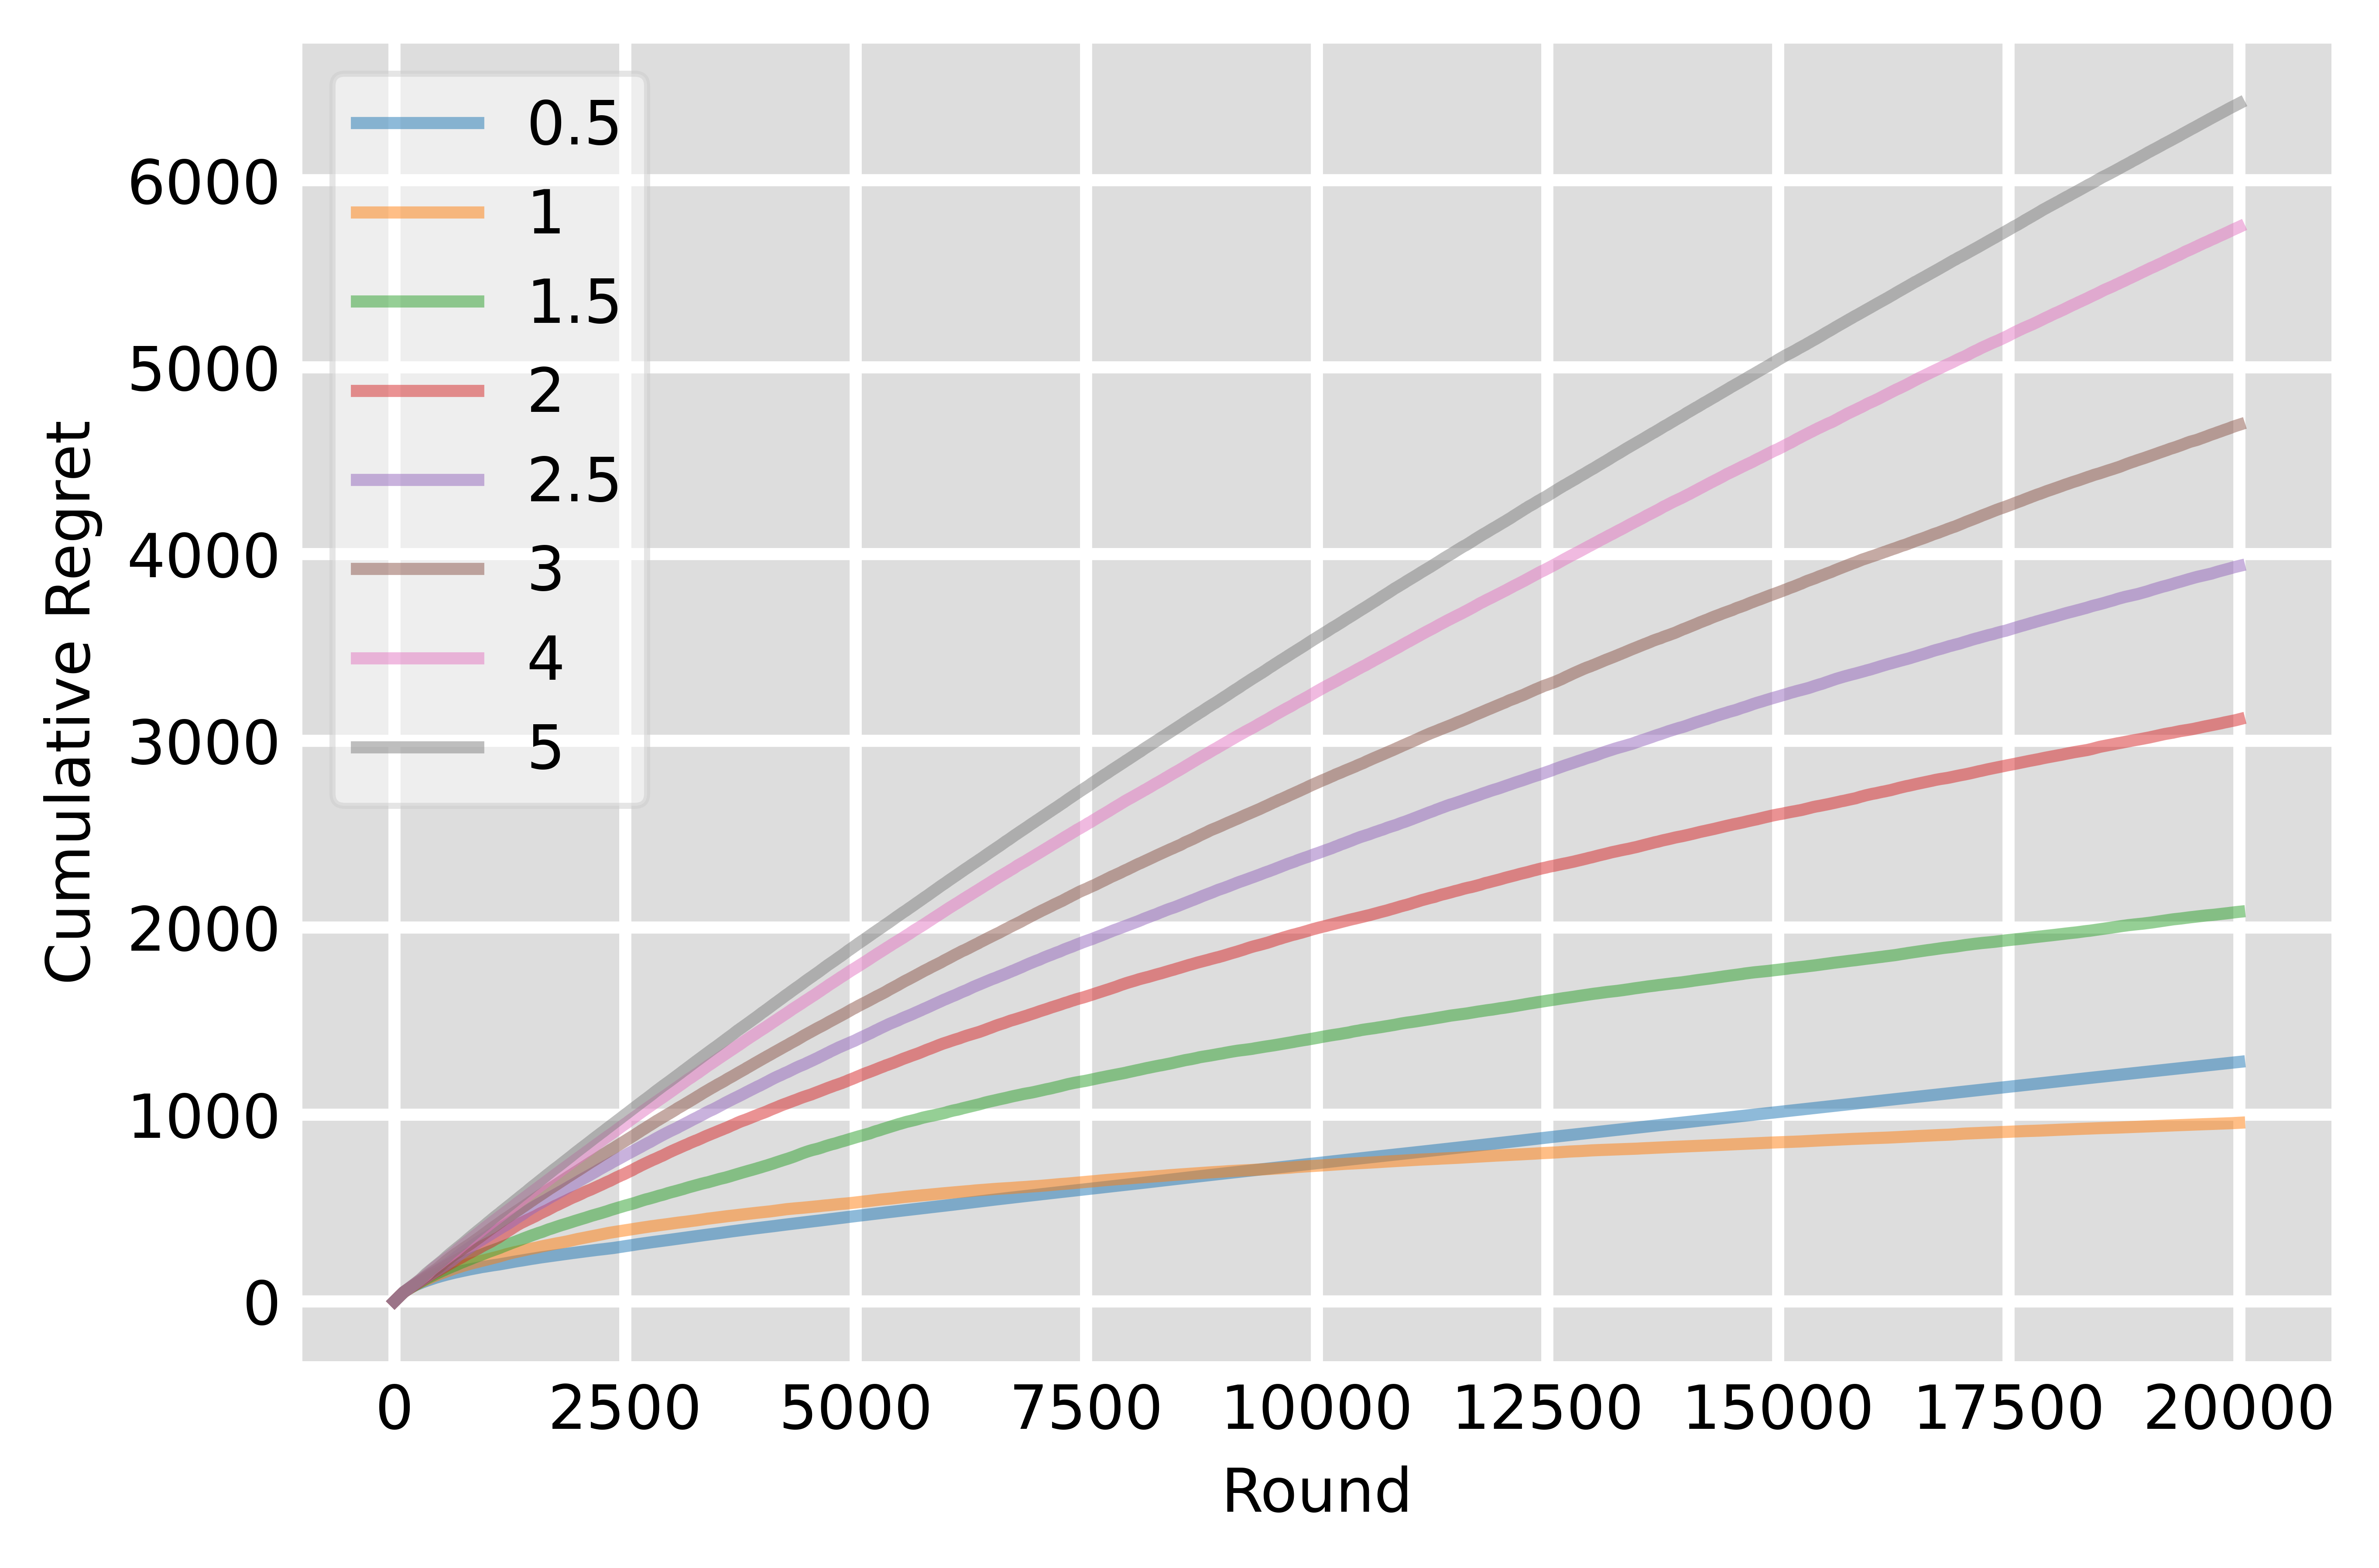
\includegraphics[width=0.9\textwidth]{figures/ucb_plot.png}
    \caption[UCB strategy with varying values of confidence level]{UCB strategy with varying values of confidence level. 100 arms. 20000 rounds per iteration. Average of 50 iterations}
    \label{fig: ucb}
\end{figure}

\begin{figure}[h]
    \centering
    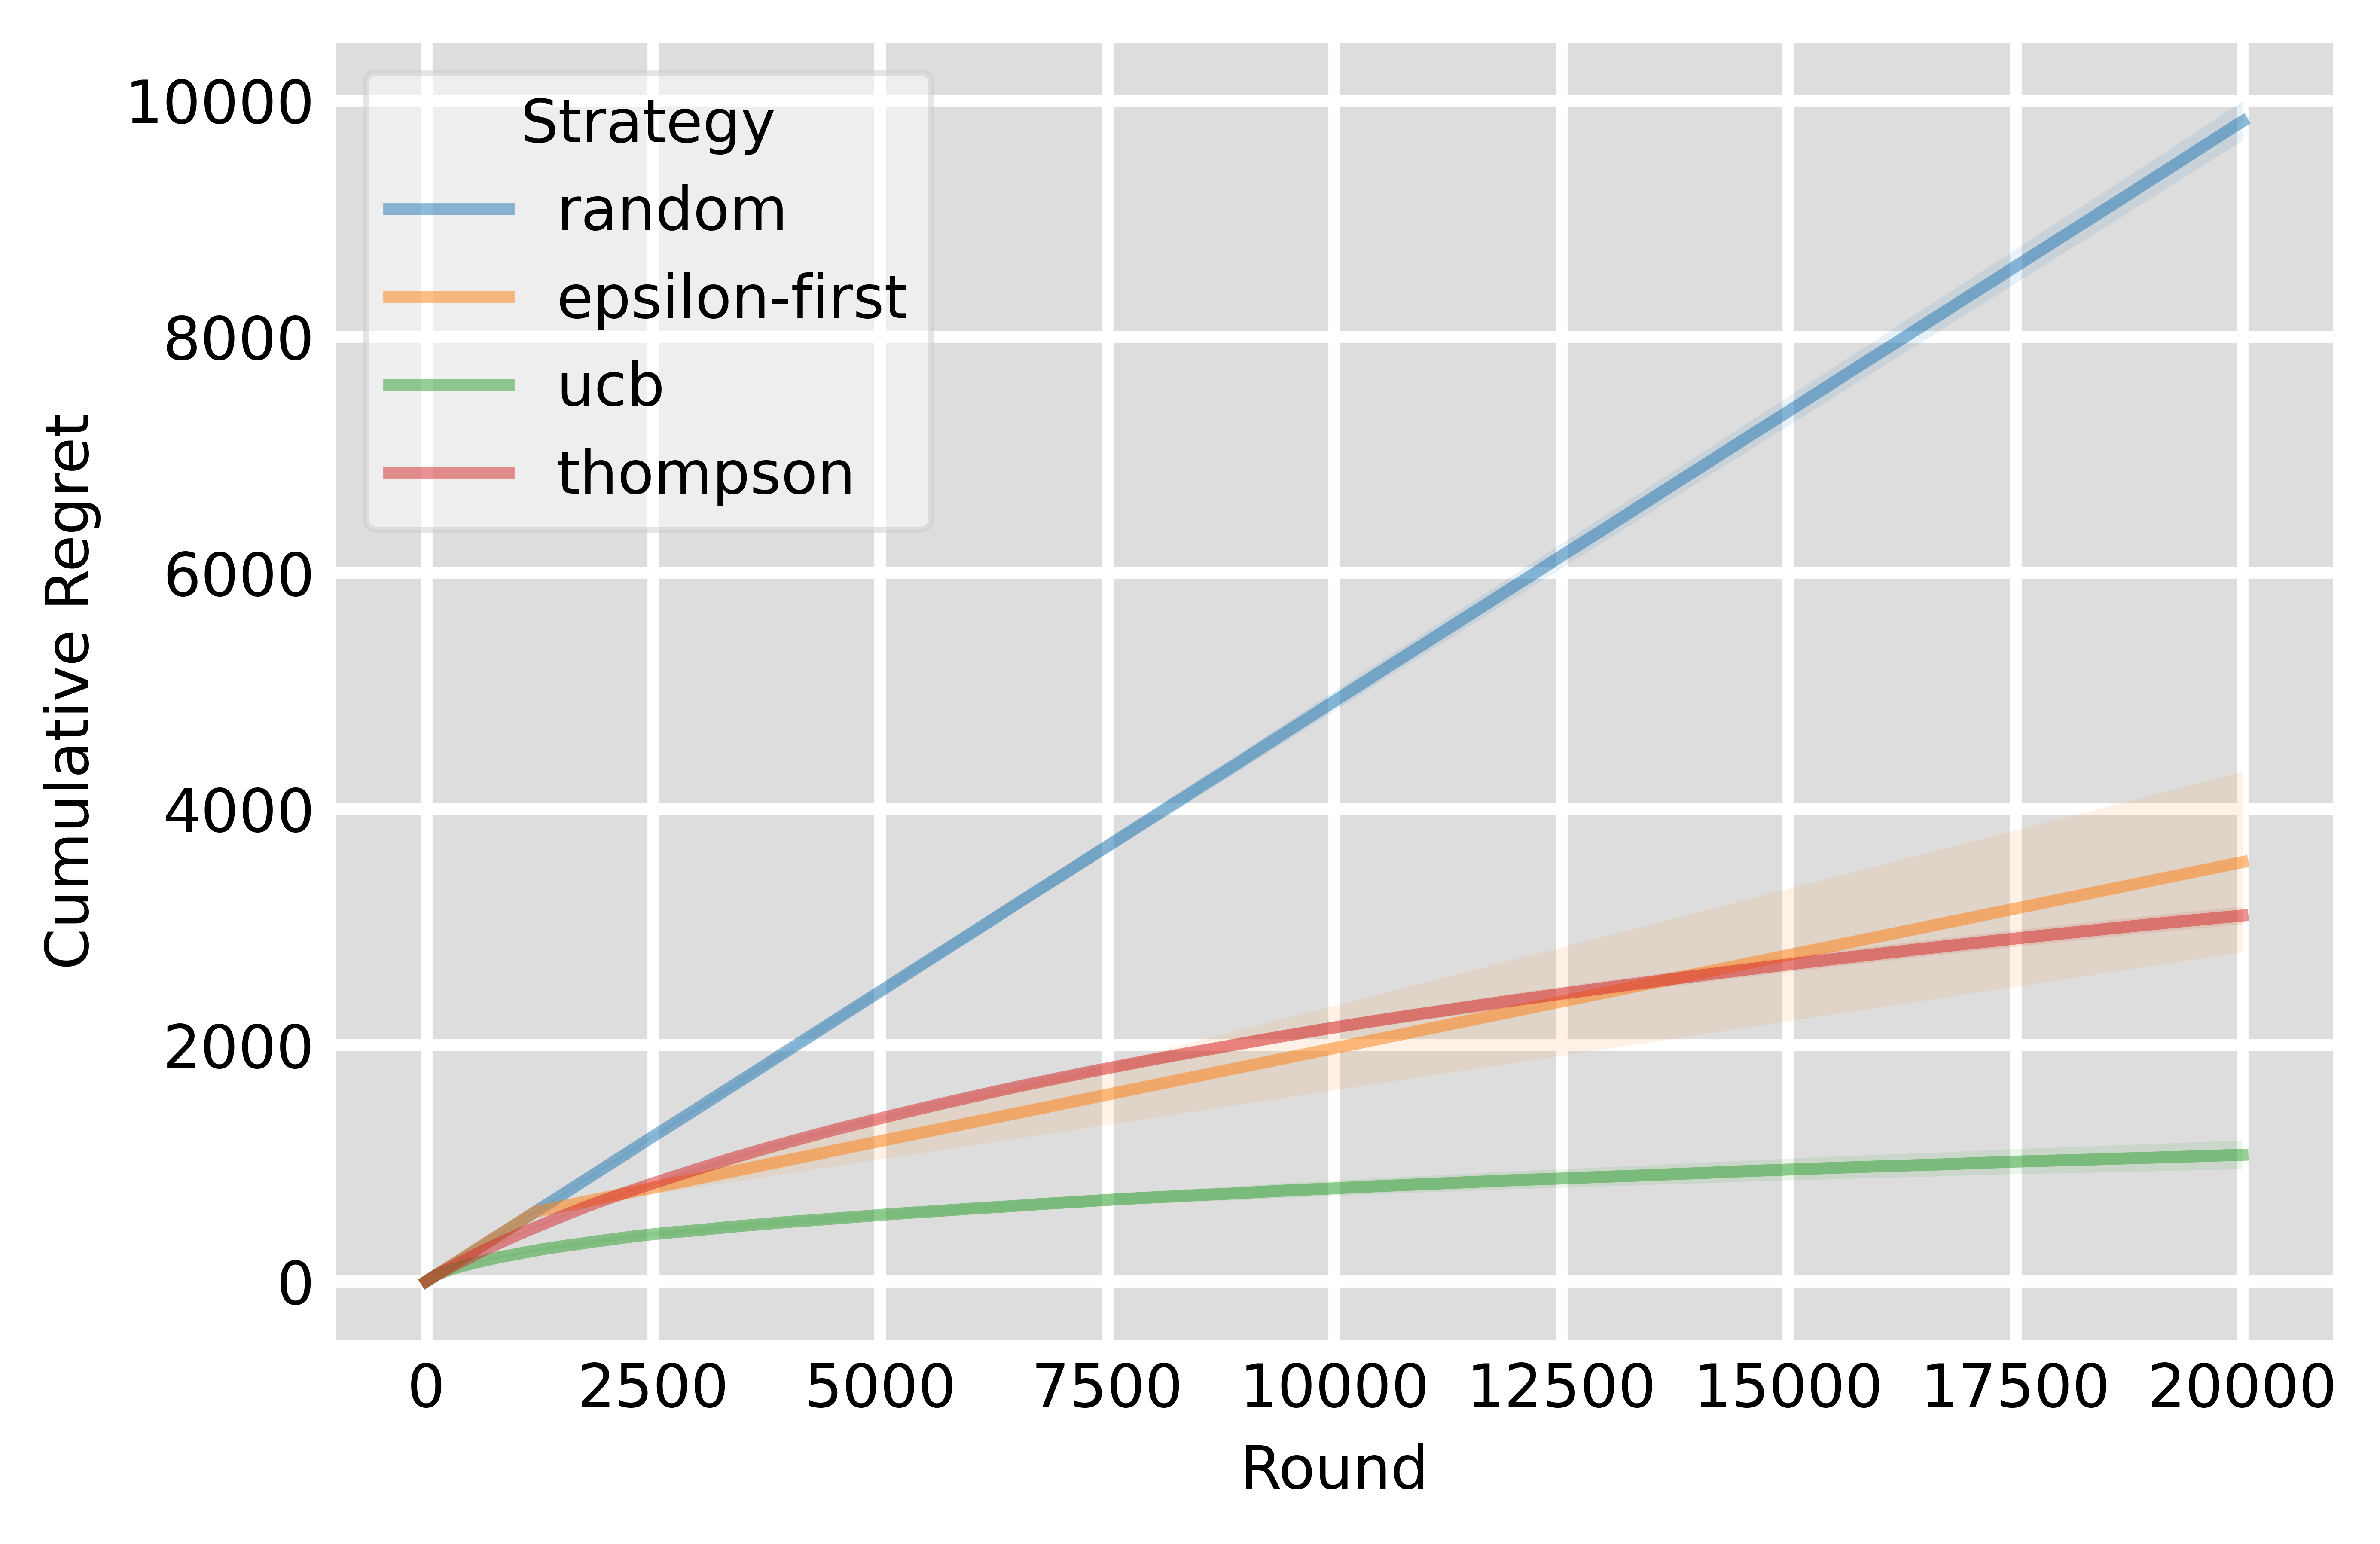
\includegraphics[width=0.9\textwidth]{figures/comparison_of_all_strategies_100_machines}
    \caption[Comparison of Stationary Strategies]{Comparison of Stationary Strategies. Epsilon =0.06, confidence level=1. 100 arms. 20000 rounds per iteration. Average of 50 iterations}
    \label{fig: all1}
\end{figure}

\begin{figure}[h]
    \centering
    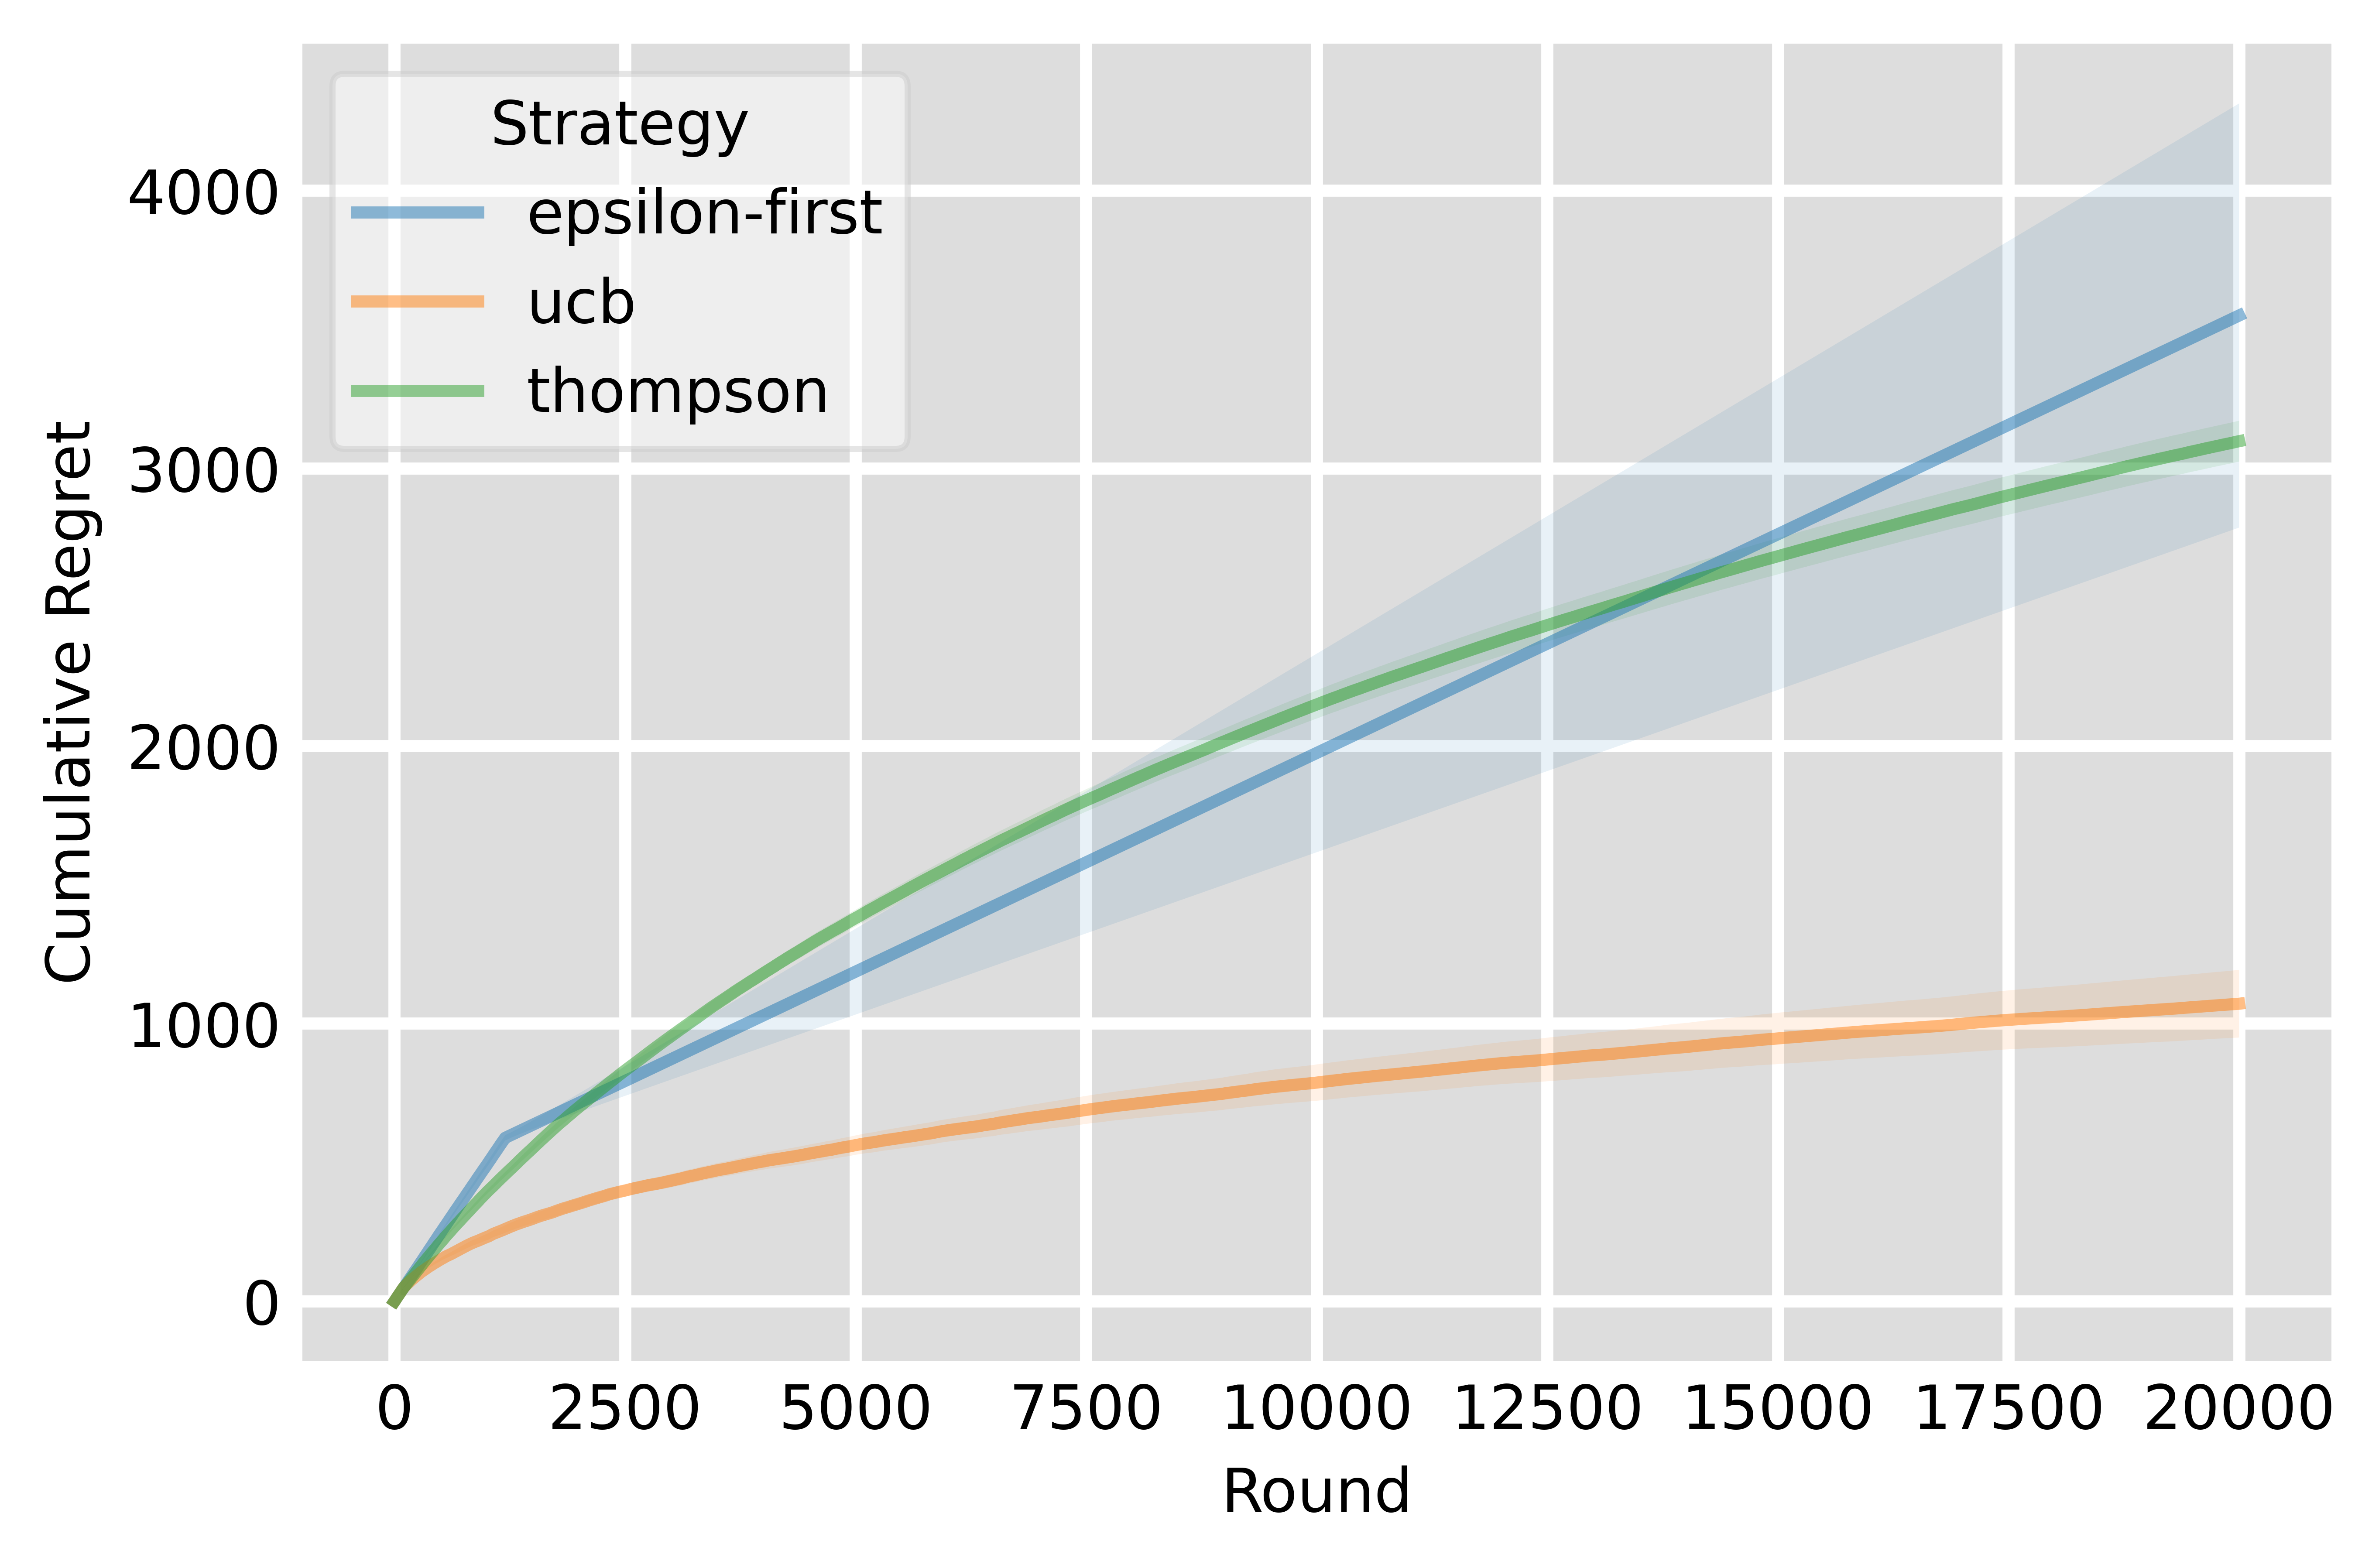
\includegraphics[width=0.9\textwidth]{figures/comparison_without_random_100_machines}
    \caption[Comparison of Stationary Strategies without random]{Comparison of Stationary Strategies without random. Epsilon =0.06, confidence level=1. 100 arms. 20000 rounds per iteration. Average of 50 iterations}
    \label{fig: 100 arms without random}
\end{figure}

\begin{figure}[h]
    \centering
    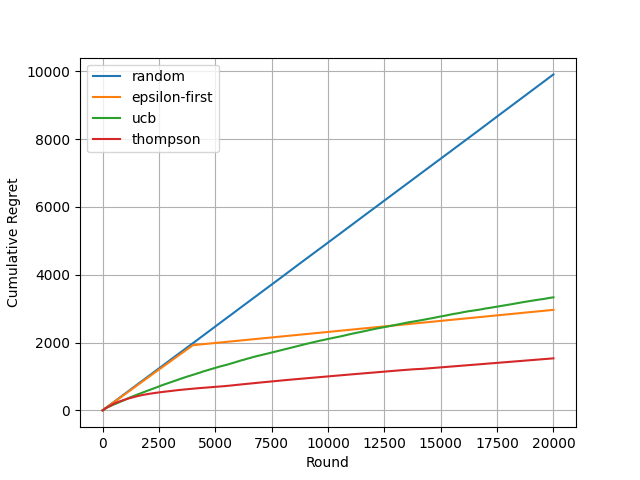
\includegraphics[width=0.9\textwidth]{figures/100machines}
    \caption[Comparison for 100 arms]{Comparison of Stationary Strategies. Epsilon =0.2, confidence level=1. 100 arms. 20000 rounds per iteration. 20 iterations}
    \label{fig: all4}
\end{figure}